\chapter{Hash Functions and Random
Oracles}\label{Hash-Functions-and-Random-Orac}

We have seen pseudorandom generators, functions and permutations, as
well as Message Authentication codes, CPA and CCA secure encryptions.
This week we will talk about cryptographic hash functions and some of
their magical properties. We motivate this by the \emph{Bitcoin}
cryptocurrency. As usual our discussion will be highly abstract and
idealized, and any resemblance to real cryptocurrencies, living or dead,
is purely coincidental.

\section{The ``Bitcoin'' Problem}\label{The-Bitcoin-Problem}

Using cryptography to create a \emph{centralized} digital-currency is
fairly straightforward, and indeed this is what is done by Visa,
Mastercard, and so on. The main challenge with Bitcoin is that it is
\emph{decentralized}. There is no trusted server, there are no ``user
accounts'', no central authority to adjudicate claims. Rather we have a
collection of anonymous and autonomous parties that somehow need to
agree on what is a valid payment.

\subsection{The Currency Problem}\label{The-Currency-Problem}

Before talking about cryptocurrencies, let's talk about currencies in
general.\footnote{I am not an economist by any stretch of the
  imagination, so please take the discussion below with a huge grain of
  salt. I would appreciate any comments on it.} At an abstract level, a
\emph{currency} requires two components:

\begin{itemize}
\item
  A scarce resource.
\item
  A mechanism for determining and transferring \emph{ownership} of
  certain quantities of this resource.
\end{itemize}

Some currencies are/were based on \href{https://goo.gl/K7awAW}{commodity
money}. The scarce resource was some commodity having intrinsic value,
such as gold or silver, or even salt or tea, and ownership based on
physical possession. However, for various financial and political
reasons, some societies shifted to
\href{https://goo.gl/K6c4qP}{representative money}, where the currency
is not the commodity itself but rather a certificate that provides the
right to the commodity. Representative money requires trust in some
central authority that would respect the certificate. The next step in
the evolution of currencies was
\href{https://en.wikipedia.org/wiki/Fiat_money}{fiat money}, which is a
currency (like today's dollar, ever since the U.S. moved off the
\href{https://goo.gl/SPN5BS}{gold standard}) that does not correspond to
any commodity, but rather only relies on trust in a central authority.
(Another example is the Roman coins, which though originally made of
silver, have underdone a continous process of
\href{https://goo.gl/ZDkGzL}{debasement} until they contained less than
two percent of it.) One advantage (sometimes disadvantage) of a fiat
currency is that it allows for more flexible monetary policy on parts of
the central authority.

\subsection{Bitcoin Architecture}\label{Bitcoin-Architecture}

Bitcoin is a fiat currency without a central authority. A priori this
seems like a contradiction in terms. If there is no trusted central
authority, how can we ensure a scarce resource? who settles claims of
ownership? and who sets monetary policy?

For instance, one problem we are particularly concerned with is the
\emph{double-spend} problem. The following scenario is a double-spend:

\begin{enumerate}
\def\labelenumi{\arabic{enumi}.}
\tightlist
\item
  Adversary \(A\) orders a pizza from Pinocchio's.
\item
  \(A\) gives Pinocchio's a particular ``set'' of money \(m\).
\item
  \(A\) eats the pizza.
\item
  \(A\) gives that same set of money \(m\) to another Domino's
  \emph{such that Pinocchio's no longer has that money}.
\item
  \(A\) eats the second pizza.
\end{enumerate}

With cash, this situation is unfathomable. But think about a credit
card: if you can ``revoke'' (or dispute) the first payment, you could
take money away from Pinocchio's \emph{after} you've received some goods
or services. Also consider that rather than giving \(m\) to Domino's in
step 4, \(A\) could just give \(m\) back to itself.

We want to make it difficult or impossible for the anyone to perform a
double-spend like this.

Bitcoin (and other cryptocurrencies) aims to provide cryptographic
solutions to this problem and more.

The basic unit in the Bitcoin system is a \emph{coin}. Each coin has a
unique identifier, and a current \emph{owner} .\footnote{This is one of
  the places where we simplify and deviate from the actual Bitcoin
  system. In the actual Bitcoin system, the atomic unit is known as a
  \emph{Satoshi} and one Bitcoin (abbreviated BTC) is \(10^8\) Satoshis.
  For reasons of efficiency, there is no individual identifier per
  Satoshi and transactions can involve transfer and creation of multiple
  Satoshis. However, conceptually we can think of atomic coins each of
  which has a unique identifier.} Transactions in the system have either
the form of ``mint coin with identifier \(\ensuremath{\mathit{ID}}\) and
owner \(P\)'' or ``transfer the coin \(\ensuremath{\mathit{ID}}\) from
\(P\) to \(Q\)''. All of these transactions are recorded in a public
\emph{ledger}.

Since there are no user accounts in Bitcoin, the ``entities'' \(P\) and
\(Q\) are not identifiers of any physical person. Rather \(P\) and \(Q\)
are ``computational puzzles''. A \emph{computational puzzle} can be
thought of as a string \(\alpha\) that specifies some ``problem'' such
that it's easy to verify whether some other string \(\beta\) is a
``solution'' for \(\alpha\), but it is hard to find such a solution on
your own. (Students with complexity background will recognize here the
class \textbf{NP}.) So when we say ``transfer the coin
\(\ensuremath{\mathit{ID}}\) from \(P\) to \(Q\)'' we mean that whomever
holds a solution for the puzzle \(Q\) is now the owner of the coin
\(\ensuremath{\mathit{ID}}\) (and to verify the authenticity of this
transfer, you provide a solution to the puzzle \(P\).) More accurately,
a transaction involving the coin \(\ensuremath{\mathit{ID}}\) is
self-validating if it contains a solution to the puzzle that is
associated with \(\ensuremath{\mathit{ID}}\) according to the latest
transaction in the ledger.

\begin{pause} \label[pause]{Please-re-read-the-previous-pa}

Please re-read the previous paragraph, to make sure you follow the
logic.

\end{pause}

One theoretical example of a puzzle is the following: if \(alpha\) is
the puzzle, an entity can ``prove'' that they own coins assigned to
\(alpha\) if they can produce numbers \(A,B\) such that \(N=A\cdot B\).

Another more generic example (that you can keep in mind as a potential
implementation for the puzzles we use here) is: \(\alpha\) is some
string in \(\{0,1\}^{2n}\) and \(\beta\) will be a string in
\(\{0,1\}^n\) such that \(\alpha = G(\beta)\) where
\(G:\{0,1\}^n\rightarrow\{0,1\}^{2n}\) is some pseudorandom generator.

The real Bitcoin system typically uses puzzles based on \emph{digital
signatures}, a concept we will learn about later in this course, but you
can simply think of \(P\) as specifying some abstract puzzle and every
person that can solve \(P\) can construct transactions with the coins
owned by \(P\).\footnote{There are reasons why Bitcoin uses digital
  signatures and not these puzzles. The main issue is that we want to
  bind the puzzle not just to the coin but also to the particular
  transaction, so that if you know the solution to the puzzle \(P\)
  corresponding to the coin \(\ensuremath{\mathit{ID}}\) and want to use
  that to transfer it to \(Q\), it won't be possible for someone to take
  your solution and use that to transfer the coin to \(Q'\) before your
  transaction is added to the public ledger. We will come back to this
  issue after we learn about digital signatures. As a quick preview, in
  Bitcoin the puzzle is as follows: whoever can produce a digital
  signature with the private key corresponding to the public key \(P\)
  can claim these coins.} Unfortunately, this means if you \emph{lose}
the solution to the puzzle then you have no access to the coin. More
alarmingly, if someone steals the solution from you, then you have no
recourse or way to get your coin back. People have managed to
\href{http://readwrite.com/2014/01/13/what-happens-to-lost-Bitcoins}{lose
millions of dollars} in this way.

\section{The Bitcoin Ledger}\label{The-Bitcoin-Ledger}

The main idea behind Bitcoin is that there is a public \emph{ledger}
that contains an ordered list of all the transactions that were ever
performed and are considered as valid in the system. Given such a
ledger, it is easy to answer the question of who owns any particular
coin. The main problem is how does a collection of anonymous parties
without any central authority agree on this ledger? This is an instance
of the \emph{consensus} problem in distributed computing. This seems
quite scary, as there are very strong negative results known for this
problem; for example the famous
\href{http://the-paper-trail.org/blog/a-brief-tour-of-flp-impossibility/}{Fischer,
Lynch Patterson (FLP) result} showed that if there is even one party
that has a \emph{benign} failure (i.e., it halts and stop responding)
then it is impossible to guarantee consensus \textbf{in a completely
asynchronous network}. Things are better if we assume some degree of
partial synchrony (i.e., a global clock and some bounds on the latency
of messages) as well as that a majority or supermajority of the parties
behave correctly.

The partial synchrony assumption is typically approximately maintained
on the Internet, but the honest majority assumption seems quite
suspicious. What does it mean a ``majority of parties'' in an anonymous
network where a single person can create multiple ``entities'' and cause
them to behave arbitrarily maliciously (known as ``byzantine'' faults in
distributed parlance)? Also, why would we assume that even one party
would behave honestly- if there is no central authority and it is
profitable to cheat then they everyone would cheat, wouldn't they?

\begin{figure}
\centering
\includegraphics[width=\textwidth, height=0.25\paperheight, keepaspectratio]{../figure/Bitcoin_ledger.jpg}
\caption{The Bitcoin ledger consists of an ordered list of transactions.
At any given point in time there might be several ``forks'' that
continue the ledger, and different parties do not necessarily have to
agree on them. However, the Bitcoin architecture is designed to ensure
that the parties corresponding to a majority of the computing power will
reach consensus on a single ledger.}
\label{ledgerfig}
\end{figure}

Perhaps the main idea behind Bitcoin is that ``majority'' will
correspond to a ``majority of computing power'', or as the
\href{https://Bitcoin.org/Bitcoin.pdf}{original Bitcoin paper} says,
``one CPU one vote'' (or perhaps more accurately, ``one cycle one
vote''). It might not be immediately clear how to implement this, but at
least it means that creating fictitious new entities (sometimes known as
a \href{https://goo.gl/jMZ7Qg}{Sybill attack} after the movie about
multiple-personality disorder) cannot help. To implement it we turn to a
cryptographic concept known as ``proof of work'' which was originally
suggested by Dwork and Naor in 1991 as a way to combat mass marketing
email.\footnote{This was a rather visionary paper in that it foresaw
  this issue before the term ``spam'' was introduced and indeed when
  email itself, let alone spam email, was hardly widespread.}

Consider a pseudorandom function \(\{ f_k \}\) mapping \(n\) bits to
\(\ell\) bits. On average, it will take a party Alice \(2^\ell\) queries
to obtain an input \(x\) such that \(f_k(x)=0^\ell\). So, if we're not
too careful, we might think of such an input \(x\) as a \emph{proof}
that Alice spent \(2^\ell\) time.

\begin{pause} \label[pause]{Stop-here-and-try-to-think-if-}

Stop here and try to think if indeed it is the case that one cannot find
an input \(x\) such that \(f_k(x)=0^\ell\) using much fewer than
\(2^\ell\) steps.

\end{pause}

The main question in using PRF's for proofs of work is who is holding
the key \(k\) for the pseudorandom function. If there is a trusted
server holding the key, then sure, finding such an input \(x\) would
take on average \(2^\ell\) queries, but the whole point of Bitcoin is to
\emph{not} have a trusted server. If we give \(k\) to a party Alice,
then can we guarantee that she can't find a ``shortcut'' to find such an
input without running \(2^\ell\) queries? The answer, in general, is
\textbf{no}.

\begin{pause} \label[pause]{Indeed-it-is-an-excellent-exer}

Indeed, it is an excellent exercise to prove that (under the PRF
conjecture) that there exists a PRF \(\{ f_k \}\) mapping \(n\) bits to
\(n\) bits and an efficient algorithm \(A\) such that \(A(k)=x\) such
that \(f_k(x)=0^\ell\).

\end{pause}

However, suppose that \(\{ f_k \}\) was somehow a ``super-strong PRF''
that would behave like a random function \emph{even to a party that
holds the key}. In this case, we can imagine that making a query to
\(f_k\) corresponds to tossing \(\ell\) independent random coins, and it
would not be feasible to obtain \(x\) such that \(f_k(x)=0^\ell\) using
much less than \(2^\ell\) cycles. Thus presenting such an input \(x\)
can serve as a ``proof of work'' that you've spent \(2^\ell\) cycles or
so. By adjusting \(\ell\) we can obtain a proof of spending \(T\) cycles
for a value \(T\) of our choice. Now if things would go as usual in this
course then I would state a result like the following:

\begin{quote}
\textbf{Theorem:} Under the PRG conjecture, there exist super strong
PRF.
\end{quote}

Where again, the ``super strong PRF'' behaves like a truly random
function \emph{even to a party that holds the key}. Unfortunately such a
result is \emph{not} known to be true, and for a very good reason. Most
natural ways to define ``super strong PRF'' will result in properties
that can be shown to be \emph{impossible to achieve}. Nevertheless, the
intuition behind it still seems useful and so we have the following
heuristic:

\begin{quote}
\textbf{The random oracle heuristic (aka ``Random oracle model'',
Bellare-Rogaway 1993):} If a ``natural'' protocol is secure when all
parties have access to a random function
\(H:\{0,1\}^n\rightarrow\{0,1\}^\ell\), then it remains secure even when
we give the parties the \emph{description} of a cryptographic hash
function with the same input and output lengths.
\end{quote}

We don't have a good characterization as to what makes a protocol
``natural'' and we do have fairly strong counterexamples to this
heuristic (though they are arguably ``unnatural''). That said, it still
seems useful as a way to get intuition for security, and in particular
to analyze Bitcoin (and many other practical protocols) we do need to
assume it, at least given current knowledge.

\hypertarget{romcaveatrem}{}
\begin{remark}[Important caveat on the random oracle model] \label[remark]{romcaveatrem}

The random oracle heuristic is very different from all the conjectures
we considered before. It is \textbf{not} a formal conjecture since we
don't have any good way to define ``natural'' and we do have examples of
protocols that are secure when all parties have access to a random
function but are \textbf{insecure} whenever we replace this random
function by \textbf{any} efficiently computable function (see the
homework exercises).

\end{remark}

\emph{Under the random oracle model}, we can now specify the ``proof of
work'' protocol for Bitcoin. Given some identifier
\(\ensuremath{\mathit{ID}}\in\{0,1\}^n\), an integer \(T \ll 2^n\), and
a hash function \(H:\{0,1\}^{2n}\rightarrow\{0,1\}^n\), the proof of
work corresponding to \(\ensuremath{\mathit{ID}}\) and \(T\) will be
some \(x\in\{0,1\}^*\) such that the first \(\lceil \log T \rceil\) bits
of \(H(\ensuremath{\mathit{ID}}\| x)\) are zero.\footnote{The actual
  Bitcoin protocol is slightly more general, where the proof is some
  \(x\) such that \(H(\ensuremath{\mathit{ID}}\|x)\), when interpreted
  as a number in \([2^n]\), is at most \(T\). There are also other
  issues about how exactly \(x\) is placed and
  \(\ensuremath{\mathit{ID}}\) is computed from past history that we
  ignore here.}

\subsection{From Proof of Work to Consensus on
Ledger}\label{From-Proof-of-Work-to-Consensu}

How does proof of work help us in achieving consensus?

We want every transaction \(t_i\) in the Bitcoin system to have a
corresponding proof of work. In particular, some proof of \(T_i\) time
``amount'' of work with respect to some identifier that is unique to
\(t_i\).

The \emph{length} of a ledger \((t_1,\ldots,t_n)\) is the sum of the
corresponding \(T_i\)'s. In other words, the \emph{length} corresponds
to the total number of cycles invested in creating this ledger. A ledger
is \emph{valid} if every transaction in the ledger of the form
``transfer the coin \(\ensuremath{\mathit{ID}}\) from \(P\) to \(Q\)''
is self-certified by a solution to \(P\).

Critically, participants (specifically \emph{miners}) in the Bitcoin
network are rewarded for adding valid entries to the ledger. In other
words, they are given Bitcoins (which are newly minted for them) for
performing the ``work'' required to add an entry to the ledger. However,
honest participants (including non-miners, people who just read the
ledger) will accept the longest known ledger as the ground truth. In
addition, Bitcoin miners are rewarded for adding entry \(i\)
\emph{after} entry \(i+100\) is added to the ledger. This gives miners
an incentive to choose the longest ledger to contribute their work
towards. To see why, consider the following rough approximation of the
incentive structure:

Remember that Bitcoin miners are rewarded for adding entry \(i\)
\emph{after} entry \(i+100\) is added to the ledger. Thus, by spending
``work'' (which directly corresponds to CPU cycles, which directly
corresponds to monetary value), miners are ``betting'' on whether a
particular ledger will ``win''. Think of yourself as a miner, and
consider a scenario in which there are two competing ledgers. Ledger 1
has length \(3\) and Ledger 2 has length \(6\). That means miners have
put roughly 2x the amount of work (= CPU cycles = money) into Ledger 2.
In order for Ledger 1 to ``win'' (from your perspective that means reach
length \(104\) to claim your prize and to become longer than Ledger 2),
you would have to perform \(3\) entries worth of work \emph{just to get
Ledger 1 to length \(6\)}. But in the meantime, other miners will
already be working on Ledger 2, further increasing its length! Thus you
want to add entries to Ledger 2.

If a ledger \(L\) corresponds to the majority of the cycles that were
available in this network then every honest party would accept it, as
any alternative ledger would be necessarily shorter. (See
\cref{ledgerfig}.)

Thus one can hope that the consensus ledger will continue to grow. (This
is a rather hand-wavy and imprecise argument, see
\href{https://eprint.iacr.org/2015/261}{this paper} for a more in depth
analysis; this is also related to the phenomenon known as
\href{https://en.wikipedia.org/wiki/Preferential_attachment}{preferential
attachment}.)

\paragraph{Cost to mine, mining pools:} Generally, if you know that
completing a \(T\)-cycle proof will get you a single coin, then making a
single query (which will succeed with probability \(1/T\)) is akin to
buying a lottery ticket that costs you a single cycle and has
probability \(1/T\) to win a single coin. One difference over the actual
lottery is that there is also some probability that you're working on
the wrong fork of the ledger, but this incentivizes people to avoid this
as much as possible. Another, perhaps even more major difference, is
that things are setup so that this is a \emph{profitable} enterprise and
the cost of a cycle is smaller than the value of \(1/T\) coins. Just
like in the lottery, people can and do gather in groups (known as
``mining pools'') where they pool together all their computing
resources, and then split the award if they win it. Joining a pool
doesn't change your expectation of winning but reduces the
\emph{variance}. In the extreme case, if everyone is in the same pool,
then for every cycle you spend you get exactly \(1/T\) coins. The way
these pools work in practice is that someone that spent \(C\) cycles
looking for an output with all zeroes, only has probability \(C/T\) of
getting it, but is very likely to get an output that begins with
\(\log C\) zeroes. This output can serve as their own ``proof of work''
that they spent \(C\) cycles and they can send it to the pool management
so they get an appropriate share of the reward.

\begin{quote}
\textbf{The real Bitcoin:} There are several aspects in which the
protocol described above differs from the real Bitcoin protocol. Some of
them were already discussed above: Bitcoin typically uses digital
signatures for puzzles (though it has a more general scripting language
to specify them), and transactions involve a number of Satoshis (and the
user interface typically displays currency is in units of BTC which are
\(10^8\) Satoshis). The Bitcoin protocol also has a formula designed to
factor in the decrease in dollar cost per cycle so that Bitcoins become
more expensive to mine with time. There is also a fee mechanism apart
from the mining to incentivize parties to add to the ledger. (The issue
of incentives in Bitcoin is quite subtle and not fully resolved, and it
is possible that parties' behavior will change with time.) The ledger
does not grow by a single transaction at a time but rather by a
\emph{block} of transactions, and there is also some timing
synchronization mechanism (which is needed, as per the consensus
impossibility results). There are other differences as well; see the
\href{https://eprint.iacr.org/2015/261}{Bonneau et al paper} as well as
the \href{https://eprint.iacr.org/2015/464}{Tschorsch and Scheuermann
survey} for more.
\end{quote}

\section{Collision Resistance Hash Functions and Creating Short
``Unique'' Identifiers}\label{Collision-Resistance-Hash-Func}

Another issue we ``swept under the carpet'' is how do we come up with
these unique identifiers per transaction. We want each transaction
\(t_i\) to be \emph{bound} to the ledger state \((t_1,\ldots,t_{i-1})\),
and so the ID of \(t_i\) should contain also the ID's all the prior
transactions. But yet we want this ID to be only \(n\) bits long.
Ideally, we could solve this if we had a \emph{one to one} mapping \(H\)
from \(\{0,1\}^N\) to \(\{0,1\}^n\) for some very large \(N\gg n\). Then
the ID corresponding to the task of appending \(t_i\) to
\((t_1,\ldots,t_{i-1})\) would simply be \(H(t_1\|\cdots\|t_i)\). The
only problem is that this is of course clearly impossible- \(2^N\) is
\emph{much} bigger than \(2^n\) and there is no one to one map from a
large set to a smaller set. Luckily we are in the magical world of
crypto where the impossible is routine and the unimaginable is
occasional. So, we can actually find a function \(H\) that is
``essentially'' one to one.

\begin{marginfigure}
\centering
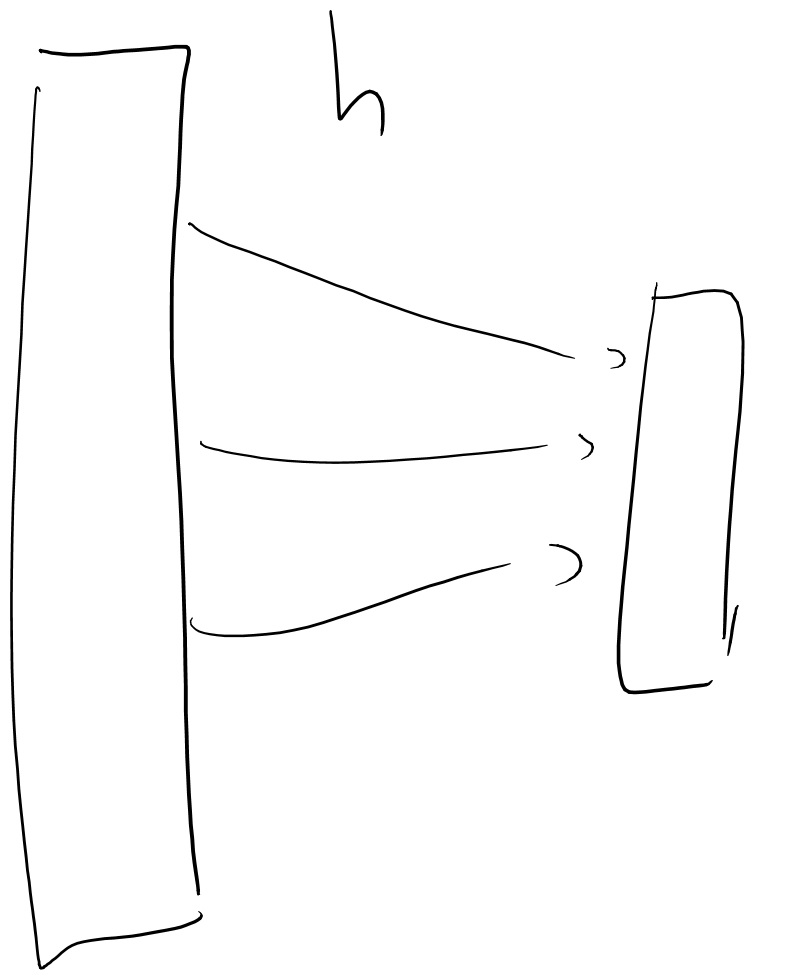
\includegraphics[width=\linewidth, height=1.5in, keepaspectratio]{../figure/hash_function.jpg}
\caption{A collision-resistant hash function is a map that from a large
universe to a small one that is ``practically one to one'' in the sense
that collisions for the function do exist but are hard to find.}
\label{tmplabelfig}
\end{marginfigure}

The main idea is the following simple result, which can be thought of as
one side of the so called \href{https://goo.gl/GSPrDW}{``birthday
paradox''}:

\hypertarget{randomcrhlem}{}
\begin{lemma} \label[lemma]{randomcrhlem}

If \(H\) is a random function from some domain \(S\) to \(\{0,1\}^n\),
then the probability that after \(T\) queries an attacker finds
\(x\neq x'\) such that \(H(x)=H(x')\) is at most \(T^2/2^n\).

\end{lemma}

\begin{proof} \label[proof]{Let-us-think-of-H-in-the-lazy-}

Let us think of \(H\) in the ``lazy evaluation'' mode where for every
query the adversary makes, we choose a random answer in \(\{0,1\}^n\) at
the time it is made. (We can assume the adversary never makes the same
query twice since a repeat query can be simulated by repeating the same
answer.) For \(i< j\) in \([T]\) let \(E_{i,j}\) be the event that
\(H(x_i)=H(x_j)\). Since \(H(x_j)\) is chosen at random and
independently from the prior choice of \(H(x_i)\), the probability of
\(E_{i,j}\) is \(2^{-n}\). Thus the probability of the union of
\(E_{i,j}\) over all \(i,j\)'s is less than \(T^2/2^n\), but this
probability is exactly what we needed to calculate.

\end{proof}

This means that a random function \(H\) is \emph{collision resistant} in
the sense that it is hard for an efficient adversary to find two inputs
that collide. Thus the random oracle heuristic would suggest that a
cryptographic hash function can be used to obtain the following object:

\hypertarget{crhdef}{}
\begin{definition}[Collision resistant hash functions] \label[definition]{crhdef}

A collection \(\{ h_k \}\) of functions where
\(h_k:\{0,1\}^*\rightarrow\{0,1\}^n\) for \(k\in\{0,1\}^n\) is a
\emph{collision resistant hash function (CRH) collection} if the map
\((k,x)\mapsto h_k(x)\) is efficiently computable and for every
efficient adversary \(A\), the probability over \(k\) that
\(A(k)=(x,x')\) such that \(x\neq x'\) and \(h_k(x)=h_k(x')\) is
negligible.\footnote{Note that the other side of the birthday bound
  shows that you can always find a collision in \(h_k\) using roughly
  \(2^{n/2}\) queries. For this reason we typically need to double the
  output length of hash functions compared to the key size of other
  cryptographic primitives (e.g., \(256\) bits as opposed to \(128\)
  bits).}

\end{definition}

Once more we do \emph{not} know a theorem saying that under the PRG
conjecture there exists a collision resistant hash function collection,
even though this property is considered as one of the desiderata for
cryptographic hash functions. However, we do know how to obtain
collections satisfying this condition under various assumptions that we
will see later in the course such as the learning with error problem and
the factoring and discrete logarithm problems. Furthermore if we
consider the weaker notion of security under a \emph{second preimage
attack} (also known as being a ``universal one way hash function'' or
UOWHF) then it \emph{is} known how to derive such a function from the
PRG assumption.

\hypertarget{crhvsprfrem}{}
\begin{remark}[CRH vs PRF] \label[remark]{crhvsprfrem}

A collection \(\{ h_k \}\) of collision resistant hash functions is an
incomparable object to a collection \(\{ f_s \}\) of pseudorandom
functions with the same input and output lengths. On one hand, the
condition of being collision-resistant does not imply that \(h_k\) is
indistinguishable from random. For example, it is possible to construct
a valid collision resistant hash function where the first output bit
always equals zero (and hence is easily distinguishable from a random
function). On the other hand, unlike \cref{prfdef}, the adversary of
\cref{crhdef} is not merely given a ``black box'' to compute the hash
function, but rather the key to the hash function. This is a much
stronger attack model, and so a PRF does not have to be collision
resistant. (Constructing a PRF that is not collision resistant is a nice
and recommended exercise.)

\end{remark}

\section{Practical Constructions of Cryptographic Hash
Functions}\label{Practical-Constructions-of-Cry}

While we discussed hash functions as \emph{keyed} collections, in
practice people often think of a hash function as being a \emph{fixed
keyless function}. However, this is because most practical constructions
involve some hardwired standardized constants (often known as IV) that
can be thought of as a choice of the key.

Practical constructions of cryptographic hash functions start with a
basic block which is known as a \emph{compression function}
\(h:\{0,1\}^{2n}\rightarrow\{0,1\}^n\). The function
\(H:\{0,1\}^*\rightarrow\{0,1\}^n\) is defined as
\(H(m_1,\ldots,m_t)=h(h(h(m_1,\ensuremath{\mathit{IV}}),m_2),\cdots,m_t)\)
when the message is composed of \(t\) blocks (and we can pad it
otherwise). See \cref{merkledamgardfig}. This construction is known as
the Merkle-Damgard construction and we know that it does preserve
collision resistance:

\begin{figure}
\centering
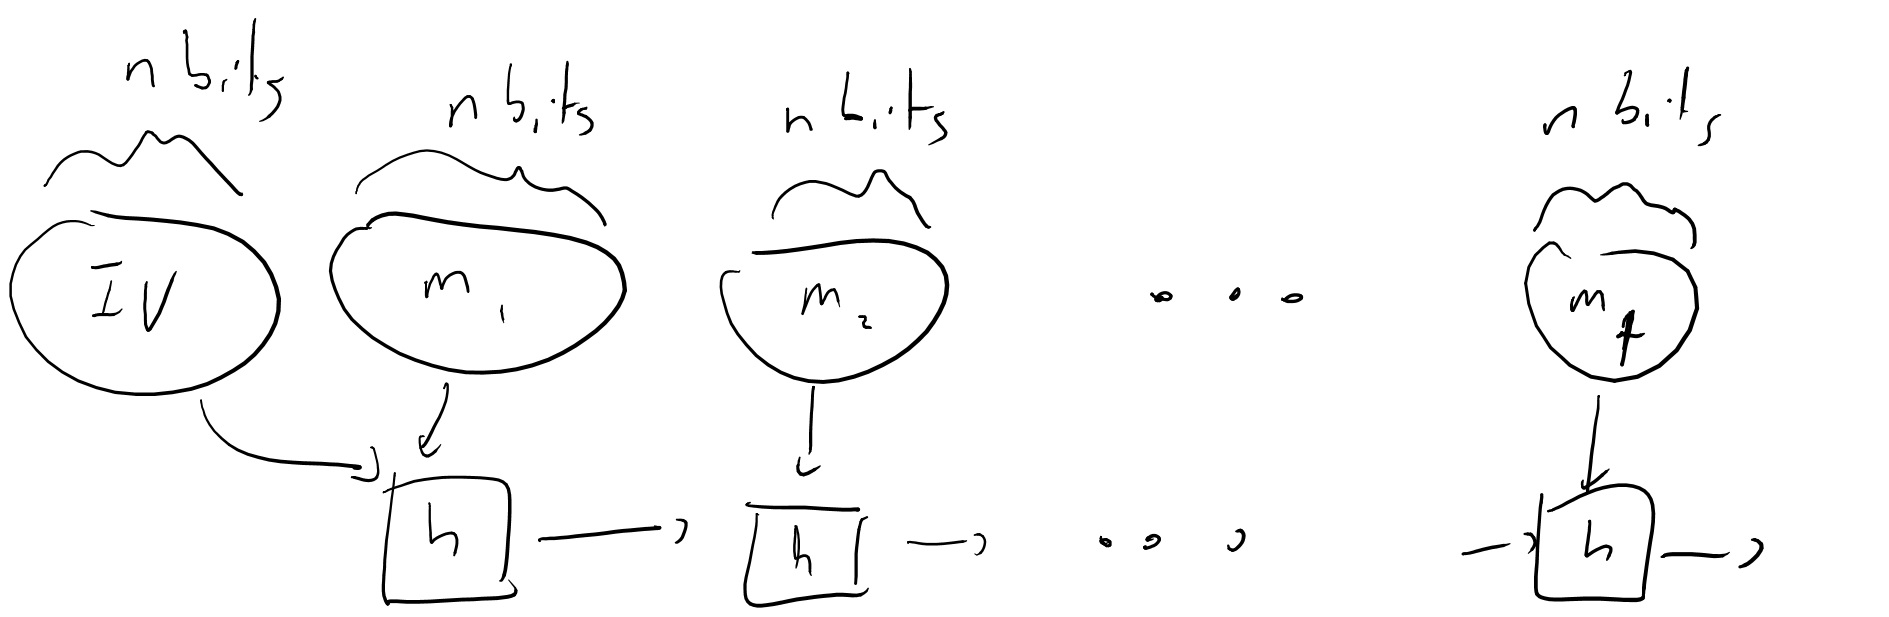
\includegraphics[width=\textwidth, height=0.25\paperheight, keepaspectratio]{../figure/merke-damgard.jpg}
\caption{The Merkle-Damgard construction converts a compression function
\(h:\{0,1\}^{2n}\rightarrow\{0,1\}^n\) into a hash function that maps
strings of arbitrary length into \(\{0,1\}^n\). The transformation
preserves collision resistance but does not yield a PRF even if \(h\)
was pseudorandom. Hence for many applications it should not be used
directly but rather composed with a transformation such as HMAC.}
\label{merkledamgardfig}
\end{figure}

\hypertarget{merkledamgardcrhthm}{}
\begin{theorem}[Merkle-Damgard preserves collision resistance] \label[theorem]{merkledamgardcrhthm}

Let \(H\) be constructed from \(h\) as above. Then given two messages
\(m \neq m' \in \{0,1\}^{tn}\) such that \(H(m)=H(m')\) we can
efficiently find two messages \(x \neq x' \in \{0,1\}^{2n}\) such that
\(h(x)=h(x')\).

\end{theorem}

\begin{proof} \label[proof]{The-intuition-behind-the-proof}

The intuition behind the proof is that if \(h\) was invertible then we
could invert \(H\) by simply going backwards. Thus in principle if a
collision for \(H\) exists then so does a collision for \(h\). Now of
course this is a vacuous statement since both \(h\) and \(H\) shrink
their inputs and hence clearly have collisions. But we want to show a
\emph{constructive} proof for this statement that will allow us to
transform a collision in \(H\) to a collision in \(h\). This is very
simple. We look at the computation of \(H(m)\) and \(H(m')\) and at the
first block in which the inputs differ but the output is the same (there
must be such a block). This block will yield a collision for \(h\).

\end{proof}

\subsection{Practical Random-ish
Functions}\label{Practical-Random-ish-Functions}

In practice we want much more than collision resistance from our hash
functions. In particular we often would like them to be PRF's as well.
Unfortunately, the Merkle-Damgard construction is \emph{not} a PRF even
when \(\ensuremath{\mathit{IV}}\) is random and secret. This is because
we can perform a \emph{length extension attack} on it. Even if we don't
know \(\ensuremath{\mathit{IV}}\), given \(y=H_{IV}(m_1,\ldots,m_t)\)
and a block \(m_{t+1}\) we can compute \(y' = h(y,m_{t+1})\) which
equals \(H_{IV}(m_1,\ldots,m_{t+1})\).

One fix for this is to use a different \(\ensuremath{\mathit{IV}}'\) in
the \emph{end} of the encryption. That is, we define:

\(H_{IV,\ensuremath{\mathit{IV}}'}(m_1,\ldots,m_t) = h(\ensuremath{\mathit{IV}}',H_{IV}(m_1,\ldots,m_t))\)

A variant of this construction (where \(\ensuremath{\mathit{IV}}'\) is
obtained as some simple function of \(\ensuremath{\mathit{IV}}\)) is
known as HMAC and it can be shown to be a pseudorandom function under
some pseudorandomness assumptions on the compression function \(h\). It
is very widely implemented. In many cases where I say ``use a
cryptographic hash function'' in this course I actually mean to use an
HMAC like construction that can be conjectured to give at least a PRF if
not stronger ``random oracle''-like properties.

The simplest implementation for a compression function is to take a
\emph{block cipher} with an \(n\) bit key and an \(n\) bit message and
then simply define
\(h(x_1,\ldots,x_{2n})=E_{x_{n+1},\ldots,x_{2n}}(x_{1},\ldots,x_{n})\).
A more common variant is known as Davies-Meyer where we also XOR the
output with \(x_{n+1},\ldots x_{2n}\). In practice people often use
\emph{tailor made} block ciphers that are designed for some efficiency
or security concerns.

\subsection{Some History}\label{Some-History}

Almost all practically used hash functions are based on the
Merkle-Damgard paradigm. Hash functions are designed to be extremely
efficient\footnote{For example, the Boneh-Shoup book quotes processing
  times of up to 255MB/sec on a 1.83 Ghz Intel Core 2 processor, which
  is more than enough to handle not just Harvard's network but even
  \href{http://www.huffingtonpost.com/2014/06/27/colleges-fastest-internet-speed-infographic_n_5536834.html}{Lamar
  College's}.} which also means that they are often at the ``edge of
insecurity'' and indeed have fallen over the edge.

In 1990 Ron Rivest proposed MD4, which was already shown weaknesses in
1991, and a full collision has been found in 1995. Even faster attacks
have been since found and MD4 is considered completely insecure.

In response to these weaknesses, Rivest designed MD5 in 1991. A weakness
was shown for it in 1996 and a full collision was shown in 2004. Hence
it is now also considered insecure.

In 1993 the National Institute of Standards proposed a standard for a
hash function known as the \emph{Secure Hash Algorithm (SHA)}, which has
quite a few similarities with the MD4 and MD5 functions. This function
is known as SHA-0, and the standard was replaced in 1995 with SHA-1 that
includes an extra ``mixing'' (i.e., bit rotation) operation. At the time
no explanation was given for this change but SHA-0 was later found to be
insecure. In 2002 a variant with longer output, known as SHA-256, was
added (as well as some others). In 2005, following the MD5 collision,
significant weaknesses were shown in SHA-1. In 2017, a
\href{https://goo.gl/jdqUX9}{full SHA-1 collision was found}. Today
SHA-1 is considered insecure and SHA-256 is recommended.

Given the weaknesses in MD-5 and SHA-1 , NIST started in 2006 a
competition for a new hashing standard, based on functions that seem
sufficiently different from the MD5/SHA-0/SHA-1 family. (SHA-256 is
unbroken but it seems too close for comfort to those other systems.) The
hash function Keccak was selected as the new standard
\href{https://goo.gl/Bx1bu2}{SHA-3} in August of 2015.

\subsection{The NSA and Hash
Functions}\label{The-NSA-and-Hash-Functions}

The NSA is the world's largest employer of mathematicians, and is very
heavily invested in cryptographic research. It seems quite possible that
they devote far more resources to analyzing symmetric primitives such as
block ciphers and hash functions than the open research community.
Indeed, the history above suggests that the NSA has consistently
discovered attacks on hash functions before the cryptographic community
(and the same holds for the differential cryptanalysis technique for
block ciphers). That said, despite the ``mythic'' powers that are
sometimes ascribed to the NSA, this history suggests that they are ahead
of the open community but not so much ahead, discovering attacks on hash
functions about 5 years or so ahead.

There are a few ways we can get ``insider views'' to the NSA's thinking.
Some such insights can be obtained from the Snowden documents. The
\href{https://en.wikipedia.org/wiki/Flame_(malware)}{Flame malware} has
been discovered in Iran in 2012 after operating since at least 2010. It
used an MD5 collision to achieve its goals. Such a collision was known
in the open literature since 2008, but Flame used a different variant
that was unknown in the literature. For this reason it is suspected that
it was designed by a western intelligence agency.

Another insight into NSA's thoughts can be found in pages 12-19 of NSA's
internal
\href{https://www.nsa.gov/public_info/_files/cryptologs/cryptolog_126.pdf}{Cryptolog
magazine} which has been recently declassified; one can find there a
rather entertaining and opinionated (or obnoxious, depending on your
point of view) review of the CRYPTO 1992 conference. In page 14 the
author remarks that certain weaknesses of MD5 demonstrated in the
conference are unlikely to be extended to the full version, which
suggests that the NSA (or at least the author) was not aware of the MD5
collisions at the time.

\subsection{Cryptographic vs Non-Cryptographic Hash
Functions}\label{Cryptographic-vs-Non-Cryptogra}

Hash functions are of course also widely used for
\emph{non-cryptographic} applications such as building hash tables and
load balancing. For these applications people often use \emph{linear}
hash functions known as \emph{cyclic redundancy codes (CRC)}. Note
however that even in those seemingly non-cryptographic applications, an
adversary might cause significant slowdown to the system if he can
generate many collisions. This can and
\href{http://arstechnica.com/business/2011/12/huge-portions-of-web-vulnerable-to-hashing-denial-of-service-attack/}{has}
been used to obtain denial of service attacks. As a rule of thumb, if
the inputs to your system might be generated by someone who does not
have your best interests at heart, you're better off using a
cryptographic hash function.
